%\documentclass{article}
%
%\usepackage{amsmath,amssymb}
%\usepackage[left=2cm, right=2cm]{geometry}
%\usepackage{tikz}

\definecolor{motive}{HTML}{800000}
\definecolor{crystalline}{HTML}{008000}
\definecolor{CSA}{HTML}{000080}

\def\ph{\vphantom{$A^A_A$}}

%\begin{document}

\noindent\hfill%
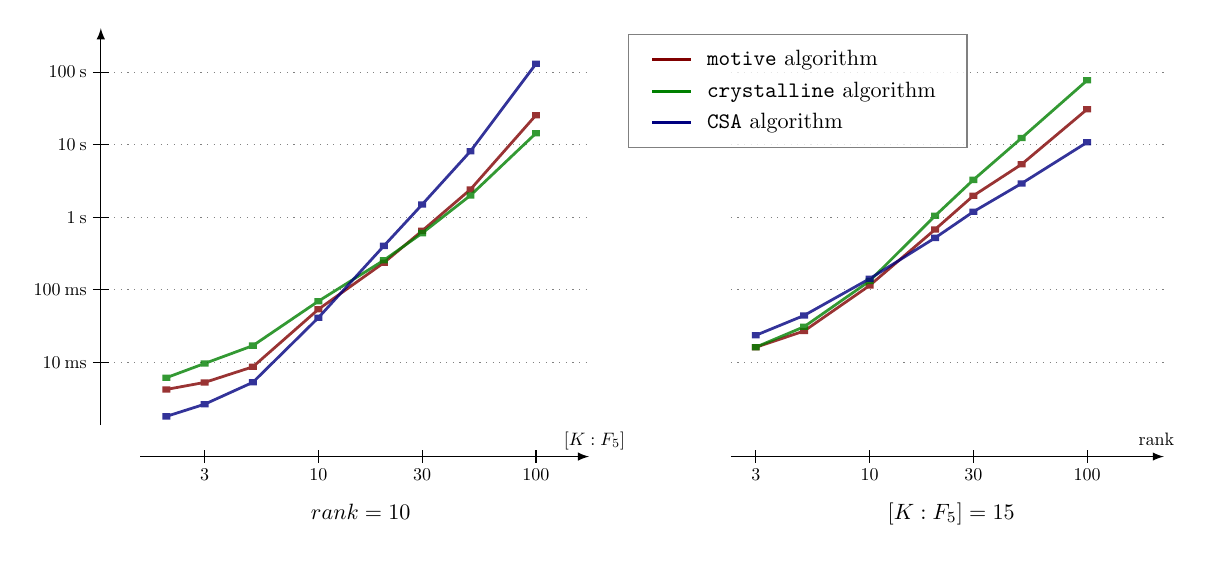
\begin{tikzpicture}[yscale=0.8]

\begin{scope}
% r = 10
% 2	0.004217s	0.006124s	0.001794s	(repeat=728)
% 3	0.005269s	0.009613s	0.002639s	(repeat=525)
% 5	0.008648s	0.016937s	0.005289s	(repeat=308)
% 10	0.053754s	0.069469s	0.041212s	(repeat=60)
% 20	0.236200s	0.255072s	0.402481s	(repeat=12)
% 30	0.649419s	0.602894s	1.498503s	(repeat=4)
% 50	2.415708s	1.996103s	8.123445s	(repeat=1)
% 100	25.520359s	14.369578s	130.432579s	(repeat=1)

\draw[-latex] (0.5,-3.8)--(6.2,-3.8);
\draw[-latex] (0,-3.3)--(0,3);
\node[above right, scale=0.65] at (5.8,-3.8) { \ph $[K:\mathbb{F}_5]$ };
\node[scale=0.8] at (3.3,-4.7) { \ph $\text{rank} = 10$ };

\draw[dotted, gray] (0,-2.303)--(6.2,-2.303);
\draw (-0.1,-2.303)--(0.1,-2.303);
\node[left,scale=0.65] at (-0.1, -2.303) { $10$\hspace{0.5ex}ms };

\draw[dotted, gray] (0,-1.151)--(6.2,-1.151);
\draw (-0.1,-1.151)--(0.1,-1.151);
\node[left,scale=0.65] at (-0.1, -1.151) { $100$\hspace{0.5ex}ms };

\draw[dotted, gray] (0,0)--(6.2,0);
\draw (-0.1,0)--(0.1,0);
\node[left,scale=0.65] at (-0.1, 0) { $1$\hspace{0.5ex}s };

\draw[dotted, gray] (0,1.151)--(6.2,1.151);
\draw (-0.1,1.151)--(0.1,1.151);
\node[left,scale=0.65] at (-0.1, 1.151) { $10$\hspace{0.5ex}s };

\draw[dotted, gray] (0,2.303)--(6.2,2.303);
\draw (-0.1,2.303)--(0.1,2.303);
\node[left,scale=0.65] at (-0.1, 2.303) { $100$\hspace{0.5ex}s };

\draw (1.318,-3.7)--(1.318,-3.9);
\node[below, scale=0.65] at (1.318,-3.9) { $3$ };

\draw (2.763,-3.7)--(2.763,-3.9);
\node[below, scale=0.65] at (2.763,-3.9) { $10$ };

\draw (4.081,-3.7)--(4.081,-3.9);
\node[below, scale=0.65] at (4.081,-3.9) { $30$ };

\draw (5.526,-3.7)--(5.526,-3.9);
\node[below, scale=0.65] at (5.526,-3.9) { $100$ };

\begin{scope}[motive, opacity=0.8, transparency group]
  \draw (0.832,-2.734)--(1.318,-2.623)--(1.931,-2.375)--(2.763,-1.462)--(3.595,-0.722)--(4.081,-0.216)--(4.694,0.441)--(5.526,1.620);
  \fill (0.782,-2.784) rectangle (0.882,-2.684);
  \fill (1.268,-2.673) rectangle (1.368,-2.573);
  \fill (1.881,-2.425) rectangle (1.981,-2.325);
  \fill (2.713,-1.512) rectangle (2.813,-1.412);
  \fill (3.545,-0.772) rectangle (3.645,-0.672);
  \fill (4.031,-0.266) rectangle (4.131,-0.166);
  \fill (4.644,0.391) rectangle (4.744,0.491);
  \fill (5.476,1.570) rectangle (5.576,1.670);
\end{scope}
\begin{scope}[crystalline, opacity=0.8, transparency group]
  \draw (0.832,-2.548)--(1.318,-2.322)--(1.931,-2.039)--(2.763,-1.333)--(3.595,-0.683)--(4.081,-0.253)--(4.694,0.346)--(5.526,1.333);
  \fill (0.782,-2.598) rectangle (0.882,-2.498);
  \fill (1.268,-2.372) rectangle (1.368,-2.272);
  \fill (1.881,-2.089) rectangle (1.981,-1.989);
  \fill (2.713,-1.383) rectangle (2.813,-1.283);
  \fill (3.545,-0.733) rectangle (3.645,-0.633);
  \fill (4.031,-0.303) rectangle (4.131,-0.203);
  \fill (4.644,0.296) rectangle (4.744,0.396);
  \fill (5.476,1.283) rectangle (5.576,1.383);
\end{scope}
\begin{scope}[CSA, opacity=0.8, transparency group]
  \draw (0.832,-3.162)--(1.318,-2.969)--(1.931,-2.621)--(2.763,-1.595)--(3.595,-0.455)--(4.081,0.202)--(4.694,1.047)--(5.526,2.435);
  \fill (0.782,-3.212) rectangle (0.882,-3.112);
  \fill (1.268,-3.019) rectangle (1.368,-2.919);
  \fill (1.881,-2.671) rectangle (1.981,-2.571);
  \fill (2.713,-1.645) rectangle (2.813,-1.545);
  \fill (3.545,-0.505) rectangle (3.645,-0.405);
  \fill (4.031,0.152) rectangle (4.131,0.252);
  \fill (4.644,0.997) rectangle (4.744,1.097);
  \fill (5.476,2.385) rectangle (5.576,2.485);
\end{scope}
\end{scope}


\begin{scope}[xshift=7cm]
% d = 15
% 3	0.016070s	0.016161s	0.023505s	(repeat=171)
% 5	0.026950s	0.030895s	0.044162s	(repeat=96)
% 10	0.114177s	0.131478s	0.141615s	(repeat=26)
% 20	0.678137s	1.045358s	0.518410s	(repeat=5)
% 30	1.977253s	3.277011s	1.189370s	(repeat=2)
% 50	5.361344s	12.371648s	2.922881s	(repeat=1)
% 100	30.792985s	77.193916s	10.774767s	(repeat=1)

\draw[-latex] (1,-3.8)--(6.5,-3.8);
\node[above right, scale=0.65] at (6.1,-3.8) { \ph rank };
\node[scale=0.8] at (3.8,-4.7) { \ph $[K:\mathbb F_5] = 15$ };

\draw[dotted, gray] (1,-2.303)--(6.5,-2.303);
\draw[dotted, gray] (1,-1.151)--(6.5,-1.151);
\draw[dotted, gray] (1,0)--(6.5,0);
\draw[dotted, gray] (1,1.151)--(6.5,1.151);
\draw[dotted, gray] (1,2.303)--(6.5,2.303);

\draw (1.318,-3.7)--(1.318,-3.9);
\node[below, scale=0.65] at (1.318,-3.9) { $3$ };

\draw (2.763,-3.7)--(2.763,-3.9);
\node[below, scale=0.65] at (2.763,-3.9) { $10$ };

\draw (4.081,-3.7)--(4.081,-3.9);
\node[below, scale=0.65] at (4.081,-3.9) { $30$ };

\draw (5.526,-3.7)--(5.526,-3.9);
\node[below, scale=0.65] at (5.526,-3.9) { $100$ };

\begin{scope}[motive, opacity=0.8, transparency group]
  \draw (1.318,-2.065)--(1.931,-1.807)--(2.763,-1.085)--(3.595,-0.194)--(4.081,0.341)--(4.694,0.840)--(5.526,1.714);
  \fill (1.268,-2.115) rectangle (1.368,-2.015);
  \fill (1.881,-1.857) rectangle (1.981,-1.757);
  \fill (2.713,-1.135) rectangle (2.813,-1.035);
  \fill (3.545,-0.244) rectangle (3.645,-0.144);
  \fill (4.031,0.291) rectangle (4.131,0.391);
  \fill (4.644,0.790) rectangle (4.744,0.890);
  \fill (5.476,1.664) rectangle (5.576,1.764);
\end{scope}
\begin{scope}[crystalline, opacity=0.8, transparency group]
  \draw (1.318,-2.063)--(1.931,-1.739)--(2.763,-1.014)--(3.595,0.022)--(4.081,0.593)--(4.694,1.258)--(5.526,2.173);
  \fill (1.268,-2.113) rectangle (1.368,-2.013);
  \fill (1.881,-1.789) rectangle (1.981,-1.689);
  \fill (2.713,-1.064) rectangle (2.813,-0.964);
  \fill (3.545,-0.028) rectangle (3.645,0.072);
  \fill (4.031,0.543) rectangle (4.131,0.643);
  \fill (4.644,1.208) rectangle (4.744,1.308);
  \fill (5.476,2.123) rectangle (5.576,2.223);
\end{scope}
\begin{scope}[CSA, opacity=0.8, transparency group]
  \draw (1.318,-1.875)--(1.931,-1.560)--(2.763,-0.977)--(3.595,-0.328)--(4.081,0.087)--(4.694,0.536)--(5.526,1.189);
  \fill (1.268,-1.925) rectangle (1.368,-1.825);
  \fill (1.881,-1.610) rectangle (1.981,-1.510);
  \fill (2.713,-1.027) rectangle (2.813,-0.927);
  \fill (3.545,-0.378) rectangle (3.645,-0.278);
  \fill (4.031,0.037) rectangle (4.131,0.137);
  \fill (4.644,0.486) rectangle (4.744,0.586);
  \fill (5.476,1.139) rectangle (5.576,1.239);
\end{scope}
\end{scope}

\begin{scope}[xshift=7cm, yshift=2.5cm, yscale=0.5]
\fill[white, opacity=0.8] (-0.3,-2.8) rectangle (4, 0.8);
\draw[gray] (-0.3,-2.8) rectangle (4, 0.8);
\draw[motive, very thick] (0,0)--(0.5,0);
\node[right, scale=0.8] at (0.6,0) { \ph \texttt{motive} algorithm };
\draw[crystalline, very thick] (0,-1)--(0.5,-1);
\node[right, scale=0.8] at (0.6,-1) { \ph \texttt{crystalline} algorithm };
\draw[CSA, very thick] (0,-2)--(0.5,-2);
\node[right, scale=0.8] at (0.6,-2) { \ph \texttt{CSA} algorithm };
\end{scope}

\end{tikzpicture}%
\hfill\null


%\end{document}
